\textbackslash{}chapter\{Hamilton's Equations\}
\textbackslash{}label\{ch:4\}

The Legendre transformation of f (a function of the us) to g (a function of
the vs) is accomplished by defining g as follows:
g =
n
i=1
uivi -f.
(4.2)
At first glance you might think that g is a function of both us and vs, but you
can appreciate that g is a function only of the vs by taking the differential of
its definition. That is,
dg =
n
i=1
(uidvi + vidui) -
n
i=1
\textbackslash{}partial f
\textbackslash{}partial ui
dui,
=
n
i=1
uidvi +
n
i=1

vi -\textbackslash{}partial f
\textbackslash{}partial ui

dui.
But by the definition of the vis (Equation (4.1)), the coefficients of the duis are
zero, so
dg =
n
i=1
uidvi,
(4.3)
and consequently g is a function only of the vs. But if dg depends only on the
vs, its differential is given by
dg = \textbackslash{}partial g
\textbackslash{}partial v1
dv1 + \textbackslash{}partial g
\textbackslash{}partial v2
dv2 + \textbackslash{}cdot  \textbackslash{}cdot  \textbackslash{}cdot  + \textbackslash{}partial g
\textbackslash{}partial vn
dvn =
n
i=1
\textbackslash{}partial g
\textbackslash{}partial vi
dvi.
(4.4)
Comparing Equations (4.3) and (4.4) we appreciate that
ui = \textbackslash{}partial g
\textbackslash{}partial vi
.
(4.5)
Note the symmetry between Equations (4.1) and (4.5). Also note that the two
functions f and g can be defined in terms of each other in a symmetrical
fashion. That is,
g =
n
i=1
uivi -f,
and
f =
n
i=1
uivi -g.
(4.6)
Essentially, that is all there is to Legendre transformations. However, it is
worth mentioning one more fact. Suppose that f also depends on some other
variables, say w1, w2, . . . , wm, that are independent of the us. Suppose, furthermore, that the ws do not participate in the transformation. We call the us
the ``active'' variables and the ws the ``passive'' variables. We have
f = f (u1, u2, . . . , un; w1, w2, . . . , wm).

4.1
The Legendre transformation
Defining the vs and g as before,
vi = \textbackslash{}partial f
\textbackslash{}partial ui
,
g =
n
i=1
uivi -f (u, w).
The differential of g is
dg =
n
i=1
(uidvi + vidui) -df,
=
n
i=1
(uidvi + vidui) -
n
i=1
\textbackslash{}partial f
\textbackslash{}partial ui
dui -

i=1
\textbackslash{}partial f
\textbackslash{}partial wi
dwi,
=
n
i=1
uidvi +
n
i=1

vi -\textbackslash{}partial f
\textbackslash{}partial ui

dui -

i=1
\textbackslash{}partial f
\textbackslash{}partial wi
dwi.
As before, the middle term on the right is zero, leaving us with
dg =
n
i=1
uidvi -

i=1
\textbackslash{}partial f
\textbackslash{}partial wi
dwi,
which indicates that g is a function of the vs and the ws. But if g = g(v, w),
its differential has the form
dg =
n
i=1
\textbackslash{}partial g
\textbackslash{}partial vi
dvi +

i=1
\textbackslash{}partial g
\textbackslash{}partial wi
dwi,
so comparing the two expressions for dg we find that
\textbackslash{}partial g
\textbackslash{}partial wi
= -\textbackslash{}partial f
\textbackslash{}partial wi
.
(4.7)
We shall soon be using this relation involving the passive variables.
\begin{exercise}
Exercise 4.1 Show that the transformation g = f -
n
i=1
uivi is also an
acceptable Legendre transformation, in the sense that g is a function only
of the vs. (This is the form used in thermodynamics.)
4.1.1 Application to thermodynamics
The Legendre transformation is particularly useful in thermodynamics.1
Without going into the definitions of the various ``thermodynamic potentials''
1 This section may be skipped without loss of continuity.

let us recall that the internal energy U is a function of entropy (S) and volume
(V ). That is, U = U(S, V ). In thermodynamics we may be interested in considering the change in U when there is a change in some variable, or perhaps
we are interested in determining the conditions under which U remains constant. For example, we might be considering a system undergoing a constant
pressure process. In general both S and V will change, and it may be difficult
to determine the effect on U. In that case it is probably more convenient to
consider the behavior of the enthalpy (H) which is a function of entropy and
pressure, H = H(S, P). If P is constant, the enthalpy is a function of only
one variable. Similarly, for a constant temperature process, we might prefer to
consider the Helmholtz free energy F = F(T, V ). If both the temperature and
pressure are constant (as in a chemistry laboratory), we might prefer to consider the Gibbs free energy G = G(T, P). These thermodynamic potentials
(U, H, F, G) are different functions of different variables, yet they are related
because they describe different aspects of the same thermodynamic system. As
you may recall from your thermodynamics course, they are obtained from one
another through Legendre transformations. For example, the familiar first law
of thermodynamics ``change in energy = heat into the system -work done by
the system'' is expressed by
dU = T dS -PdV.
But since U = U(S, V )
dU = \textbackslash{}partial U
\textbackslash{}partial S dS + \textbackslash{}partial U
\textbackslash{}partial V dV,
so we appreciate that T = \textbackslash{}partial U/\textbackslash{}partial S and P = -\textbackslash{}partial U/\textbackslash{}partial V. Using these facts we
can generate the other thermodynamic potentials by Legendre transformations.
For example, F is a function depending on T and V. We generate F by simply
using the prescription of Exercise 4.1,
F = U -T S.
To show that F is indeed a function of T and V we note that
dF = dU -T dS -SdT
= T dS -PdV -T dS -SdT
= -PdV -SdT.
Therefore F = U -T S is indeed a function of T and V .

4.2
Application to the Lagrangian. The Hamiltonian
\end{exercise}

\begin{exercise}
Exercise 4.2 In the transformation described above, from internal energy
to Helmholtz free energy, identify the active variables and the passive variables.
\end{exercise}

\begin{exercise}
Exercise 4.3 Given dU
=
T dS -PdV, determine H(S, P) and
G(T, P). Answers: H = U + PV, G = U -T S + PV.
4.2 Application to the Lagrangian. The Hamiltonian
We now apply the Legendre transformation to the Lagrangian. The Lagrangian
is a function of qi, $\textbackslash{}dot q$i, t
L = L(q1, . . . , qn; $\textbackslash{}dot q$1, . . . , $\textbackslash{}dot q$n; t).
In our Legendre transformation we shall let the $\textbackslash{}dot q$s be the active variables and
the qs and t be the passive variables. Therefore, the new function will depend
on the qs and t and on the derivatives of L with respect to the $\textbackslash{}dot q$s. If the new
function is denoted by H we have
H = H(qi, \textbackslash{}partial L/\textbackslash{}partial $\textbackslash{}dot q$i, t).
But we know that \textbackslash{}partial L/\textbackslash{}partial $\textbackslash{}dot q$i = pi, the generalized momentum conjugate to qi.
Therefore, the new function will be
H = H(qi, pi, t).
We define H by the usual prescription for a Legendre transformation
(Equation (4.2)), obtaining
H(qi, pi, t) =
n
i=1
pi $\textbackslash{}dot q$i -L(qi, $\textbackslash{}dot q$i, t).
(4.8)
The function H is called the Hamiltonian. We shall see shortly that in many
situations it is equal to the total energy.
Keep in mind that the Hamiltonian must be expressed in terms of the generalized momentum. An expression for H involving velocities is wrong. You
may consider Equation (4.8) as a definition of the Hamiltonian. (It would be a
good idea to memorize it.)
\end{exercise}

\begin{exercise}
Exercise 4.4 Determine H for a free particle using Equation (4.8).
(Answer: H = (p2
x + p2
y + p2
z)/2m.)

\end{exercise}

\begin{exercise}
Exercise 4.5 The Lagrangian for a disk rolling down an inclined plane is
L = 1
2m $\textbackslash{}dot y$2 + 1
4mR2 $\textbackslash{}dot\textbackslash{}$theta 2 + mg(y -l) sin \textbackslash{}alpha .
(See Example 3.1.) What is the Hamiltonian for this system? (Answer:
H = p2
y/2m + p2
\textbackslash{}theta /mR2 -Mg(y -R) sin \textbackslash{}alpha .)
4.3 Hamilton's canonical equations
The Hamiltonian is the function of qi, pi, t that was obtained from the
Lagrangian by assuming that the $\textbackslash{}dot q$is are the active variables and that the qis
and t are the passive variables. Therefore, expressing Equations (4.1) and (4.5)
in terms of the variables introduced in the previous section we have
pi = \textbackslash{}partial L
\textbackslash{}partial $\textbackslash{}dot q$i
and
$\textbackslash{}dot q$i = \textbackslash{}partial H
\textbackslash{}partial pi
.
(4.9)
Furthermore, from the relations among the passive variables given in Equations (4.7) we have
\textbackslash{}partial H
\textbackslash{}partial qi
= -\textbackslash{}partial L
\textbackslash{}partial qi
and
\textbackslash{}partial H
\textbackslash{}partial t = -\textbackslash{}partial L
\textbackslash{}partial t .
(4.10)
Now the Lagrange equation tells us that
dt
\textbackslash{}partial L
\textbackslash{}partial $\textbackslash{}dot q$i

= \textbackslash{}partial L
\textbackslash{}partial qi
.
That is,
$\textbackslash{}dot p$i = \textbackslash{}partial L
\textbackslash{}partial qi
.
Therefore, substituting for \textbackslash{}partial L/\textbackslash{}partial qi from the first of Equations (4.10) we have
$\textbackslash{}dot p$i = -\textbackslash{}partial H
\textbackslash{}partial qi
.
(4.11)
This equation and the second equation of (4.9) give us the following two
extremely important relations:
$\textbackslash{}dot q$i = \textbackslash{}partial H
\textbackslash{}partial pi
,
(4.12)
$\textbackslash{}dot p$i = -\textbackslash{}partial H
\textbackslash{}partial qi
.
(4.13)

4.3
Hamilton's canonical equations
These are called ``Hamilton's canonical equations.'' They are the equations of
motion of the system expressed as 2n first-order differential equations. They
have the very nice property that the derivatives with respect to time are isolated
on the left-hand sides of the equation.
I will now present yet another way to obtain the canonical equations. We
begin with the definition
H(qi, pi, t) =
n
i=1
pi $\textbackslash{}dot q$i -L(qi, $\textbackslash{}dot q$i, t).
(4.14)
Evaluating the partial derivative of the Hamiltonian with respect to the generalized coordinate qi yields
\textbackslash{}partial H
\textbackslash{}partial qi
=
\textbackslash{}partial
\textbackslash{}partial qi

pi $\textbackslash{}dot q$i -L(qi, $\textbackslash{}dot q$i, t)

= -\textbackslash{}partial L
\textbackslash{}partial qi
= -d
dt
\textbackslash{}partial L
\textbackslash{}partial $\textbackslash{}dot q$i
= -$\textbackslash{}dot p$i.
(4.15)
Here we have used Lagrange's equations and the definition of generalized
momentum. Next, we take the partial derivative of the Hamiltonian with respect
to the generalized momentum pi:
\textbackslash{}partial H
\textbackslash{}partial pi
=
\textbackslash{}partial
\textbackslash{}partial pi

pi $\textbackslash{}dot q$i -L(qi, $\textbackslash{}dot q$i, t)

= $\textbackslash{}dot q$i.
(4.16)
Equations (4.15) and (4.16) give us, once again, the canonical equations of
motion:
\textbackslash{}partial H
\textbackslash{}partial qi
= -$\textbackslash{}dot p$,
(4.17)
\textbackslash{}partial H
\textbackslash{}partial pi
= $\textbackslash{}dot q$i.
Since H is also a function of time, let us take the partial derivative of Equation (4.14) with respect to time. This yields immediately the interesting result
\textbackslash{}partial H
\textbackslash{}partial t = -\textbackslash{}partial L
\textbackslash{}partial t .
(4.18)
Consider the total time derivative of the Hamiltonian. It is
dH(q, p, t)
dt
= \textbackslash{}partial H
\textbackslash{}partial q
dq
dt + \textbackslash{}partial H
\textbackslash{}partial p
dp
dt + \textbackslash{}partial H
\textbackslash{}partial t
= -$\textbackslash{}dot p$ dq
dt + $\textbackslash{}dot q$ dp
dt + \textbackslash{}partial H
\textbackslash{}partial t
= -$\textbackslash{}dot p$ $\textbackslash{}dot q$ + $\textbackslash{}dot q$ $\textbackslash{}dot p$ + \textbackslash{}partial H
\textbackslash{}partial t = \textbackslash{}partial H
\textbackslash{}partial t ,

where we used Hamilton's equations. And so
dH
dt = \textbackslash{}partial H
\textbackslash{}partial t .
(4.19)
Comparing Equations (4.18) and (4.19) we conclude that if the Lagrangian is
not an explicit function of time, the Hamiltonian is constant. Furthermore, if
the transformation equations do not depend explicitly on time and if the potential energy depends only on the coordinates, then the Hamiltonian is the total
energy. In quantum mechanical problems one is often required to write down
and solve the Schrödinger equation. This requires an expression for the
Hamiltonian. Often people simply write H = T + V for the Hamiltonian,
and most of the time this is correct. However, you should be aware that there
are situations in which the Hamiltonian is not the total energy of the system.
\end{exercise}

\begin{exercise}
Exercise 4.6 Consider a frictionless harmonic oscillator consisting of a
mass m on a spring of constant k, as in Section 1.10.2. Obtain the Hamiltonian, evaluate the canonical equations, and solve for the position as a
function of time. (Answer: $\textbackslash{}dot p$ = -kx and $\textbackslash{}dot x$ = px/m.)
4.4 Derivation of Hamilton's equations from
Hamilton's principle
Hamilton's equations can also be derived by considering Hamilton's principle
which states that the time development of a mechanical system is such that the
action integral is stationary. That is,
\textbackslash{}delta I = \textbackslash{}delta
t2
t1
Ldt = 0.
We have shown that this leads to Lagrange's equations. We now show that this
principle also leads to Hamilton's equations. Recall that the Lagrangian formulation treats the time development of a mechanical system as the motion
of a point in configuration space. The Hamiltonian formulation treats the time
development of a mechanical system as the motion of a point in phase space.
For a system of N particles, phase space is a 6N-dimensional space in which
the axes are labelled qi, pi, (i = 1, . . . , n), where n = 3N. In the Hamiltonian formulation the momenta and the coordinates are on an equal footing as
variables. (See Section 1.8.)
To obtain Hamilton's equations from Hamilton's principle, it must be formulated in terms of the ps and qs. Therefore, we use the definition of the

4.5
Phase space and the phase fluid
Hamiltonian as given by Equation (4.8) and write Hamilton's principle as
\textbackslash{}delta I = \textbackslash{}delta
t2
t1
Ldt = \textbackslash{}delta
t2
t1

pi $\textbackslash{}dot q$i -H(qi, pi, t)

dt = 0.
(4.20)
When written in this form, it is usually referred to as the ``modified Hamilton's
principle.'' Note that this is an expression of the form
\textbackslash{}delta I = \textbackslash{}delta
t2
t1
f (q, $\textbackslash{}dot q$, p, $\textbackslash{}dot p$, t)dt = 0.
We know from the calculus of variations that this condition can be met if and
only if the 2n Euler--Lagrange equations are satisfied. These equations have
the form
dt
\textbackslash{}partial f
\textbackslash{}partial $\textbackslash{}dot q$i

-\textbackslash{}partial f
\textbackslash{}partial qi
= 0,
i = 1, . . . , n,
and
dt
\textbackslash{}partial f
\textbackslash{}partial $\textbackslash{}dot p$i

-\textbackslash{}partial f
\textbackslash{}partial pi
= 0,
i = 1, . . . , n.
Carrying out the indicated partial differentiations we obtain
\textbackslash{}partial H
\textbackslash{}partial qi
= -$\textbackslash{}dot p$,
\textbackslash{}partial H
\textbackslash{}partial pi
= $\textbackslash{}dot q$i.
That is, we have derived Hamilton's equations from the variational principle.
\end{exercise}

\begin{exercise}
Exercise 4.7 Carry out the partial differentiation indicated above to obtain
Hamilton's canonical equations.
\end{exercise}

\section*{4.5  Phase space and the phase fluid}

The action integral expressed in terms of the Hamiltonian is
I =
t2
t1
n

i=1
pi $\textbackslash{}dot q$i -H(q1, . . . qn, p1 . . . pn, t)

dt.
When expressed in this way (as a function of qs and ps) it is called the ``canonical integral.'' As we have just seen, setting the variation of this integral to
zero yields the canonical equations $\textbackslash{}dot p$i = -\textbackslash{}partial H/\textbackslash{}partial qi and $\textbackslash{}dot q$i = +\textbackslash{}partial H/\textbackslash{}partial pi.

y
Possible trajectories for a projectile whose initial configuration space
location (0, 0) is specified but whose initial velocity is not specified.
The system is now described in terms of the 2n variables, qi and pi, for i =
1, . . . , n. The system can be represented as a point C in the 2n-dimensional
space called phase space. (We usually refer to both the ps and qs as ``coordinates.'') As time goes on, point C traces out a curve in phase space.
Recall that previously we considered the system to be represented by a single
point in configuration space. (Configuration space is the n-dimensional space
made up of the qs.)
Suppose that we wanted to consider all possible paths starting from some
initial point in configuration space. Since the velocity is not specified, if we
consider all possible velocities, we would have an infinite number of curves
\begin{figure}[h]
\centering
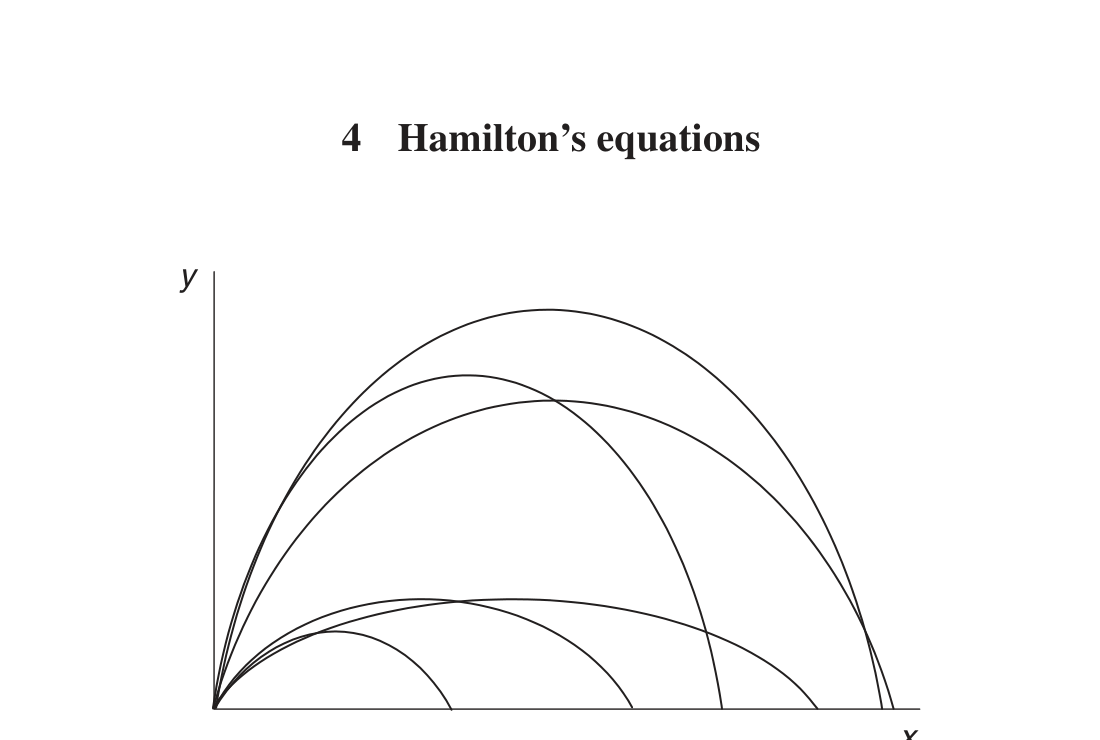
\includegraphics[width=0.55\linewidth]{../Figures/fig_4_1.png}
\caption{Figure 4.1}
\end{figure}

the possible trajectories of a projectile that starts from the origin but whose
velocity is not specified. Note specifically that the trajectories that originate at
a specific point in configuration space will, in general, cross trajectories that
originate at that point with a different velocity (as well as those that originate
at nearby points in configuration space).2
On the other hand, if we consider all possible curves from a point in phase
space we get a single curve because the point C now includes the momentum
of the particle as well as its position, thus giving the initial direction of motion
and the initial speed. The paths from other points will not cross the path from
our original point because the canonical equations define a unique slope at each
point in phase space. (When two trajectories cross, they have different slopes
at the point of intersection.)
2 We are usually not interested in a particular solution corresponding to some special initial
conditions, but rather, a general solution that is valid for arbitrary initial conditions. The
particular solution will be a single trajectory in configuration space, but for the general
solution we obtain an infinite number of trajectories.

4.5
Phase space and the phase fluid
The totality of phase space curves originating from every point in phase
space can be considered to be the general solution of the dynamical problem with each curve representing the motion for a particular set of initial
conditions.
A different way to consider the phase space curves is to suppose that the
system is made up of a great many particles. At some initial time, each particle
will be at a specific point in phase space and as time goes on, each particle will
trace out a curve in phase space. It is easy to picture this as analogous to the
motion of water molecules in a flowing river. At some initial time, each water
molecule has a specific location and a specific momentum. As time goes on
the water molecules trace out streamlines that do not cross each other.
This analogy is so good that we can apply concepts of fluid dynamics to
phase space and talk about the properties of the ``phase fluid.''
For example, the velocity of the phase fluid at every point is given by the
canonical equations, $\textbackslash{}dot p$i = -\textbackslash{}partial H/\textbackslash{}partial qi and $\textbackslash{}dot q$i = +\textbackslash{}partial H/\textbackslash{}partial pi. This can be interpreted as analogous to the velocity field in a real fluid. Each streamline of the
moving phase fluid represents the time development of the system for given
specific initial conditions and the motion of the phase fluid as a whole represents the complete solution, that is, the time development of the system for
arbitrary initial conditions.
In fluid dynamics we are especially interested in steady fluid flows. We say
that a fluid flow is steady if the velocity at a point is constant in time, that
is, the velocity field does not depend on t. If the flow of our phase fluid is
steady, then $\textbackslash{}dot p$i and $\textbackslash{}dot q$i are constants in time and the quantities \textbackslash{}partial H/\textbackslash{}partial qi and
\textbackslash{}partial H/\textbackslash{}partial pi are independent of time, and H cannot contain time explicitly. That
is, \textbackslash{}partial H/\textbackslash{}partial t = 0. But the total time derivative of H is
dH
dt =
n

i=1
\textbackslash{}partial H
\textbackslash{}partial qi
$\textbackslash{}dot q$i + \textbackslash{}partial H
\textbackslash{}partial pi
$\textbackslash{}dot p$i

= 0,
by the canonical equations. So
dH
dt = 0 =\textbackslash{}implies H = constant = E.
That is, energy is conserved. Furthermore, H = E defines a surface in phase
space and a particle will move on that surface. We conclude that, if energy is
conserved, the phase fluid behaves like the steady flow of a real fluid.
As we shall see in the next chapter, there is another analogy between real
fluids and the phase fluid; namely, the phase fluid will be shown to behave like
an incompressible real fluid.

\section*{4.6  Cyclic coordinates and the Routhian procedure}

If a coordinate does not appear in the Lagrangian it is called cyclic or ignorable.
However, the Lagrangian is still a function of the corresponding generalized
velocity. In other words, if one of the qs is ignorable, then the Lagrangian is a
function of only n -1 generalized coordinates, but it is in general a function
of all n of the generalized velocities. Thus, if qn is ignorable,
L = L(q1, . . . , qn-1; $\textbackslash{}dot q$1, . . . , $\textbackslash{}dot q$n; t).
However, the Hamiltonian will be a function of only n -1 of the coordinates and n -1 of the momenta, because the momentum conjugate to an
ignorable coordinate is constant. For example, if qn is ignorable, the corresponding momentum, pn is a constant. Let us call it \textbackslash{}alpha . We can then write the
Hamiltonian as
H = H(q1, . . . , qn-1; p1, . . . , pn-1; \textbackslash{}alpha ; t),
(4.21)
where we have included the constant \textbackslash{}alpha  in our expression even though one
normally does not express the functional dependence on a constant. It is true,
however, that H does depend on the value assigned to \textbackslash{}alpha .
The ignorable coordinate qn does not appear in the Hamiltonian, but this
does not mean that we are not interested in its time development. An ignorable
coordinate is still a coordinate on the same footing as any other! Hamilton's
equation for qn is, as you might expect,
$\textbackslash{}dot q$n = \textbackslash{}partial H
\textbackslash{}partial \textbackslash{}alpha  .
It often happens that some of the coordinates are ignorable and others are
not. For example, let us assume that a system described by the coordinates
q1, . . . , qn is such that the first s coordinates appear in the Hamiltonian (and
Lagrangian) but the coordinates qs+1, . . . , qn are cyclic. In that case a procedure for handling such problems (which was developed by Routh) can come
in handy. One defines a quantity called the Routhian (which is similar in some
respects to the Hamiltonian) as follows:
R =
n

i=s+1
pi $\textbackslash{}dot q$i -L.
(4.22)
Note that the summation is over the cyclic coordinates. Thus,
R = R(q1, . . . , qs; $\textbackslash{}dot q$1, . . . , $\textbackslash{}dot q$s; ps+1, . . . , pn; t).

4.6
Cyclic coordinates and the Routhian procedure
Taking partial derivatives of the Routhian with respect to the variables, we find
\textbackslash{}partial R
\textbackslash{}partial qi
= -\textbackslash{}partial L
\textbackslash{}partial qi
,
i = 1, . . . , s,
(4.23)
\textbackslash{}partial R
\textbackslash{}partial $\textbackslash{}dot q$i
= -\textbackslash{}partial L
\textbackslash{}partial $\textbackslash{}dot q$i
,
i = 1, . . . , s,
and
\textbackslash{}partial R
\textbackslash{}partial qi
= -$\textbackslash{}dot p$i,
i = s + 1, . . . , n,
(4.24)
\textbackslash{}partial R
\textbackslash{}partial pi
= $\textbackslash{}dot q$i,
i = s + 1, . . . , n.
Equations (4.23) indicate that the first s coordinates obey Lagrange's equations
but with the Routhian for the Lagrangian, thus,
dt
\textbackslash{}partial R
\textbackslash{}partial $\textbackslash{}dot q$i

-\textbackslash{}partial R
\textbackslash{}partial qi
= 0,
i = 1, . . . , s,
whereas Equations (4.24) indicate that the remaining coordinates and momenta
obey Hamilton's equation with the Routhian as the Hamiltonian. But note that
for the cyclic coordinates s + 1, . . . , n the momenta are constants and we can
replace the n -s momenta by the constants \textbackslash{}alpha 1, . . . , \textbackslash{}alpha n-s. The Routhian then
can be written
R = R(q1, . . . , qs; $\textbackslash{}dot q$1, . . . , $\textbackslash{}dot q$s; \textbackslash{}alpha 1, . . . , \textbackslash{}alpha n-s; t).
(4.25)
The \textbackslash{}alpha s can be determined from initial conditions, and we have effectively
reduced the number of variables in the problem from n to s. Reducing the
number of variables is a powerful technique for solving a problem. (When we
study canonical transformations we shall encounter a method for reducing the
number of variables to zero!)
The Routhian is also convenient for analyzing steady motion. We define
steady motion as motion in which the non-cyclic variables are constant. An
example of steady motion is a planet moving in a circular orbit. In polar coordinates the Lagrangian is
L = 1
2m$\textbackslash{}dot r$2 + 1
2mr2 $\textbackslash{}dot\textbackslash{}$theta 2 + k
r .
For a circular orbit, the non-cyclic coordinate r is constant. The coordinate
\textbackslash{}theta  is cyclic and it increases linearly with time. The linear increase of cyclic
coordinates is a characteristic of steady motion as can be appreciated from the
equations of motion.

As another example, if we write the Lagrangian for a spinning, precessing top or gyroscope, we find that the only non-cyclic variable is the polar
angle \textbackslash{}theta . If the top is nutating, then \textbackslash{}theta  is no longer constant and the top ``nods''
as it precesses. This can be called ``oscillation about steady motion.''
In terms of our present discussion, the non-cyclic variables are constant.
For a system with a Routhian of the form of Equation (4.25), the equations of
motion for the cyclic coordinates (Equations (4.24)) tell us that
$\textbackslash{}dot q$i = $\textbackslash{}dot q$i(q1, . . . , qs; $\textbackslash{}dot q$1, . . . , $\textbackslash{}dot q$s; \textbackslash{}alpha 1, . . . , \textbackslash{}alpha n-s),
i = s + 1, . . . , n.
For steady motion, q1, . . . , qs are constant and $\textbackslash{}dot q$1, . . . , $\textbackslash{}dot q$s are zero, so $\textbackslash{}dot q$i
(i \textgreater{} s) = constant and hence qi(i \textgreater{} s) varies linearly with time.
\begin{exercise}
Exercise 4.8 Write the Hamiltonian for a spherical pendulum. Identify all
cyclic coordinates. Write the Routhian.
\end{exercise}

\begin{exercise}
Exercise 4.9 Write the Lagrangian for a spinning top in terms of Euler
angles and identify the cyclic and non-cyclic coordinates.
\end{exercise}

\section*{4.7  Symplectic notation}

Symplectic notation is an elegant and powerful way of expressing Hamilton's
equations using matrices. One begins by defining a column matrix \textbackslash{}eta  whose
elements are all the qs and all the ps. Specifically, for a system with n degrees
of freedom, the first n elements in \textbackslash{}eta  are q1, . . . , qn, and the remaining n elements are p1, . . . , pn. Thus \textbackslash{}eta  has 2n elements. Next we define another 2n
column matrix whose elements are the partial derivatives of the Hamiltonian
with respect to all the coordinates and all the momenta so that the elements of
this column matrix are
\textbackslash{}partial H
\textbackslash{}partial q1
, \textbackslash{}partial H
\textbackslash{}partial q2
, . . . , \textbackslash{}partial H
\textbackslash{}partial qn
, \textbackslash{}partial H
\textbackslash{}partial p1
, \textbackslash{}partial H
\textbackslash{}partial p2
, . . . , \textbackslash{}partial H
\textbackslash{}partial pn
.
We shall denote this matrix by
\textbackslash{}partial H
\textbackslash{}partial \textbackslash{}eta  .
Finally, we define a 2n \textbackslash{}times  2n matrix called J which has the form
J =
-1

,

4.8
Problems
where 0 represents the n\textbackslash{}times n zero matrix and 1 represents the n\textbackslash{}times n unit matrix.
Using this notation, Hamilton's equations are
$\textbackslash{}dot\textbackslash{}$eta  = J\textbackslash{}partial H
\textbackslash{}partial \textbackslash{}eta  .
(4.26)
It might be noted that such an expression lends itself to rapid computerized
calculations. Computer programs that evaluate such equations of motion are
referred to as ``symplectic integrators'' and are widely used in celestial mechanics (for the many body problem) as well as in molecular dynamics and accelerator physics.
\begin{exercise}
Exercise 4.10 Show that Equation (4.26) reproduces Hamilton's equations for the simple harmonic oscillator of Exercise 4.6.
\end{exercise}

\section*{4.8  Problems}

4.1 Write the Hamiltonian for the double planar pendulum.
\section*{4.2  Consider the following Lagrangian:}

L = A$\textbackslash{}dot x$2 + B $\textbackslash{}dot y$ + C $\textbackslash{}dot x$ $\textbackslash{}dot y$ +

x2 + y2 ,
where A, B, C, D are constants. Determine the Hamiltonian.
\section*{4.3  A plane pendulum of length l and mass m is suspended in such a way}

that its point of support moves uniformly in a vertical circle of radius a.
Obtain Hamilton's equations of motion. What is the canonical momentum?
\section*{4.4  Obtain the Hamiltonian for a planet in orbit about the Sun in plane polar}

coordinates. Determine Hamilton's equations of motion.
4.5 Obtain the Hamiltonian and Hamilton's equations of motion for a spherical pendulum.
4.6 Express Hamilton's equations of motion for a spherical pendulum in
symplectic notation.
\section*{4.7  A particle of mass m is constrained to move on the surface of a sphere}

of radius R (until it falls off). The potential energy of the particle is mgz,
where z is measured vertically from the plane on which the sphere is
resting. Write the Hamiltonian and Hamilton's equations of motion for
the time the particle is in contact with the sphere.
4.8 Consider a canonical transformation. Write the functional determinant
and show that 2 = 1. (The functional determinant is a determinant

whose elements are partial derivatives of one set of variables with respect
to another set. Each row contains derivatives of only one variable and
each column contains derivatives with respect to only one variable.)
\section*{4.9  A massless spring of constant k is suspended from a point of support that}

oscillates vertically at a frequency \textbackslash{}omega  such that the position of the top of
the spring is given by z0 = A cos \textbackslash{}omega t. A particle of mass m is attached to
the lower end of the spring. Determine the Hamiltonian of the system.
4.10 A particle of mass m can slide freely on a horizontal rod of mass M. One
end of the rod is attached to a turntable and moves in a circular path of
radius a at angular speed \textbackslash{}omega . Write the Hamiltonian for the system.

In this chapter we begin by considering canonical transformations. These are
transformations that preserve the form of Hamilton's equations. This is followed by a study of Poisson brackets, an important tool for studying
canonical transformations. Finally we consider infinitesimal canonical transformations and, as an example, we look at angular momentum in terms of
Poisson brackets.
\section*{5.1  Integrating the equations of motion}

In our study of analytical mechanics we have seen that the variational principle leads to two different sets of equations of motion. The first set consists
of the Lagrange equations and the second set consists of Hamilton's canonical
equations. Lagrange's equations are a set of n coupled second-order differential equations and Hamilton's equations are a set of 2n coupled first-order
differential equations.
The ultimate goal of any dynamical theory is to obtain a general solution for
the equations of motion. In Lagrangian dynamics this requires integrating the
equations of motion twice. This is often quite difficult because the Lagrangian
(and hence the equations of motion) depends not only on the coordinates but
also on their derivatives (the velocities). There is no known general method
for integrating these equations.1 You might wonder if it is possible to transform to a new set of coordinates in which the equations of motion are simpler and easier to integrate. Indeed, this is possible in some situations. But the
Lagrangian is L = T -V with T a function of velocities and V a function of
1 Of course we can always carry out a numerical integration, but that depends on selecting a
particular set of initial conditions so we do not obtain a general solution.